\documentclass[11pt]{article}
\usepackage[a4paper,margin=24mm]{geometry}
\usepackage[T1]{fontenc}
\usepackage{lmodern,microtype,amsmath,amssymb,amsthm,mathtools,mathrsfs}
\usepackage{booktabs,array,graphicx,xcolor,enumitem,fancyhdr}
\usepackage[colorlinks=true,linkcolor=teal!65!black,citecolor=teal!65!black,urlcolor=teal!65!black]{hyperref}
\definecolor{ink}{HTML}{153044}
\definecolor{accent}{HTML}{087F8C}
\setlength{\parindent}{0pt}
\setlength{\parskip}{5pt}
\setlength{\headheight}{15pt}
\pagestyle{fancy}\fancyhf{}
\fancyhead[L]{\small On Quantum Mechanics and General Relativity}
\fancyhead[R]{\small Logan Voss}
\fancyfoot[C]{\thepage}
\newtheorem{theorem}{Theorem}[section]
\newtheorem{proposition}[theorem]{Proposition}
\newtheorem{corollary}[theorem]{Corollary}
\newcommand{\Tr}{\operatorname{Tr}}
\newcommand{\sech}{\operatorname{sech}}
\newcommand{\arcosh}{\operatorname{arcosh}}
\newcommand{\dd}{\mathrm d}
\newcommand{\R}{\mathbb R}
\hypersetup{pdftitle={On Quantum Mechanics and General Relativity},pdfauthor={Logan Voss},pdfsubject={Conditional action selection, quantum geometry, and reproducible verification}}
\begin{document}
\hypersetup{pageanchor=false}
\begin{titlepage}
\vspace*{12mm}
{\color{accent}\small\scshape Research edition 1.0}\par
\vspace{10mm}
{\color{ink}\Huge\bfseries On Quantum Mechanics\par and General Relativity}\par
\vspace{9mm}
{\Large Logan Voss}\par
\vspace{9mm}
{\large An exact quantum-geometric bridge\par in a two-symmetry gravitational model}\par
\vspace{10mm}
\hrule\vspace{6mm}
\textbf{The central result.} Requiring one explicitly flat reference geometry to be stationary under independent metric, area, and shape variations selects
\[
\boxed{F(\rho)=a\rho+b,\qquad U(\rho)=\frac{a}{2\rho},\qquad
W(\rho)=a\rho,\qquad V(\rho)=0.}
\]
The selected bulk action is the two-Killing reduction of Einstein gravity. Its shape geometry is exactly the geometry of centered, uncertainty-saturating canonical quantum states, with a specified normalization and frame identification.
\par\vspace{4mm}
\textbf{This edition adds} finite-distance quantum fidelity, the Berry-curvature interpretation of the invariant boundary term, complete coefficient-residual bounds, and an exact nonlinear solver benchmark. The research proof build contains 48 theorems in eight Lean modules and completes with zero warnings and zero errors.
\vfill
{\small November 13, 2026\par
Independent research with AI-assisted mathematical development, verification, formalization, and editing. Mathematical derivations were completed before public authoring. Synthetic computations are distinguished from physical observations throughout.}\par
\end{titlepage}
\hypersetup{pageanchor=true}

\begin{abstract}
We present a conditional selection theorem linking canonical quantum-state geometry to a symmetry-restricted gravitational action. Centered one-mode states saturating the Robertson--Schr\"odinger covariance bound determine positive unimodular matrices with hyperbolic information geometry. A calibrated common frame representation identifies these matrices with the shape of two spacelike symmetry orbits. Within a local invariant action class of total derivative order at most two, full first-variation stationarity of a Milne--polar flat-space chart selects the affine coefficient family and a constant parity-odd coupling. An off-shell identity identifies the selected bulk action with reduced Einstein--Hilbert gravity. We make explicit the associated finite-distance fidelity and Berry-curvature formulas, complete sharp pointwise coefficient-inference bounds, integrate them into near-affine estimates, and test the nonlinear evolution against an exact geodesic/Bessel solution. The accompanying bundle preserves the source lineage and provides 48 compiled Lean theorems, exact symbolic checks, independent quadratures, and bounded numerical convergence controls. The geometric dictionary and theory-class assumptions remain inputs. The results establish an exact model-level connection, with a reproducible proof and computation chain; interacting continuum quantization and empirical applicability remain separate obligations.
\end{abstract}
\tableofcontents
\newpage

\section{The question and the model}
The question is whether a local gravitational action can be selected by consistency requirements rather than by choosing its coefficient functions in advance. The answer here is exact within a specified model. The word \emph{stationary} has its variational meaning: the first variation vanishes. It does not mean that every perturbation stays small for all time.

Let $B$ be an oriented two-dimensional Lorentzian base, $h$ a metric of signature $(-,+)$, $\rho>0$ an area field, and $M$ a symmetric positive $2\times2$ matrix with determinant one. The literal metric dictionary is
\begin{equation}\label{eq:dictionary}
g=h_{ab}(x)\dd x^a\dd x^b+\rho(x)M_{IJ}(x)\dd y^I\dd y^J.
\end{equation}
The two $y$ directions are commuting spacelike symmetry directions. There are no mixed base--orbit connection fields. Dimension, Lorentzian base signature, orbit labels, and their calibration are supplied. The resulting model retains nonlinear shape dynamics while restricting the gravitational sector.

Write
\begin{equation}
J_a=M^{-1}\partial_aM,\quad T_{ab}=\Tr(J_aJ_b),\quad
\tau=h^{ab}T_{ab},\quad X=h^{ab}\rho_a\rho_b.
\end{equation}
In global target coordinates,
\begin{equation}\label{eq:target}
M(P,Q)=\begin{pmatrix}e^P&e^PQ\\e^PQ&e^{-P}+e^PQ^2\end{pmatrix},
\qquad G=\tfrac12\Tr[(M^{-1}\dd M)^2]=\dd P^2+e^{2P}\dd Q^2.
\end{equation}
Its invariant area form is $\Omega=e^P\dd P\wedge\dd Q=\dd(e^P\dd Q)$.

Assume locality, base diffeomorphism invariance, constant target $SL(2,\R)$ congruence invariance, the stated field content, and polynomial dependence on derivatives of \emph{total order at most two}. Modulo divergences, the action is
\begin{align}
S_{\mathrm{even}}&=\int_B\sqrt{-h}\left[F(\rho)R[h]+U(\rho)X-\frac{W(\rho)}4\tau+V(\rho)\right]\dd^2x,\label{eq:action}\\
S_{\mathrm{odd}}&=2\int_B k(\rho)e^P(P_tQ_r-P_rQ_t)\dd t\dd r.\label{eq:odd}
\end{align}
Here $F\in C^2(0,\infty)$ and $U,W,V,k\in C^1(0,\infty)$. The target isotropy representation has no invariant covector and has one symmetric and one alternating invariant bilinear form up to scale. This removes independent mixed area--shape terms and leaves precisely the displayed functions. A term $C(\rho)\Box\rho$ integrates into $U$. The full classification and variation are preserved in the v2.4 supplement~\cite{Voss24}.

Total derivative order is essential. Merely requiring second-order field equations would allow a larger class, including nonlinear powers of first-derivative invariants.

\section{Full stationarity selects the affine family}
\begin{theorem}[Conditional action selection]\label{thm:selection}
For the action \eqref{eq:action}--\eqref{eq:odd}, vary all independent fields before evaluating the reference chart
\begin{equation}\label{eq:chart}
h=-\dd t^2+\dd r^2,\quad \rho=tr,\quad P=\log(t/r),\quad Q=0,\qquad t,r>0.
\end{equation}
Stationarity for every smooth compactly supported variation on every relatively compact regular subdomain is equivalent to
\begin{equation}\label{eq:selected}
F=a\rho+b,\quad U=\frac a{2\rho},\quad W=a\rho,\quad V=0,\quad k=k_0,
\end{equation}
with common constants on the connected positive area domain. Positive nondegenerate shape energy further selects $a>0$.
\end{theorem}

\begin{proof}
The metric variation of the even action is
\begin{equation}\label{eq:metricEL}
\begin{split}
E_{ab}={}&(h_{ab}\Box-\nabla_a\nabla_b)F
+U(\rho_a\rho_b-\tfrac12h_{ab}X)\\
&-\frac W4(T_{ab}-\tfrac12h_{ab}\tau)-\tfrac12h_{ab}V.
\end{split}
\end{equation}
The two-dimensional Einstein tensor vanishes identically, while the displayed derivatives of $F$ remain. The even area and shape equations are
\begin{align}
E_\rho^{\mathrm{even}}&=F'R-U'X-2U\Box\rho-\tfrac14W'\tau+V',\label{eq:areaEL}\\
E_P^{\mathrm{even}}&=\nabla_a(W\nabla^aP)-We^{2P}(\nabla Q)^2,\\
E_Q^{\mathrm{even}}&=\nabla_a(We^{2P}\nabla^aQ).
\end{align}
The variation is performed before gauge specialization, so the trace-free metric equations are retained.

On \eqref{eq:chart}, $\Box\rho=0$, $X=t^2-r^2$, and
\[
T_{tt}=2/t^2,\quad T_{rr}=2/r^2,\quad T_{tr}=-2/\rho,
\qquad \tau=2X/\rho^2.
\]
Set $s_0=t^2+r^2$. The three metric components become
\begin{align}
E_{tt}&=-F''t^2+\tfrac12Us_0-\frac{Ws_0}{4\rho^2}+\tfrac12V,\label{eq:tt}\\
E_{rr}&=-F''r^2+\tfrac12Us_0-\frac{Ws_0}{4\rho^2}-\tfrac12V,\label{eq:rr}\\
E_{tr}&=-(\rho F''+F')+\rho U+\frac W{2\rho}.\label{eq:tr}
\end{align}
Subtracting the first two equations gives $V=F''(t^2-r^2)$. Fix any $\rho>0$. The point $(\sqrt\rho,\sqrt\rho)$ gives $V(\rho)=0$; the point $(2\sqrt\rho,\sqrt\rho/2)$ gives $(15\rho/4)F''(\rho)=0$. The remaining components then yield
\[
F''=0,\qquad V=0,\qquad 2\rho^2U=W,\qquad W=\rho F'.
\]
The mean-value theorem applied to $F'$ on every compact segment makes $F'=a$ on the connected domain. Applying it again to $F-a\rho$ gives $F=a\rho+b$.

The odd term is metric independent. On the calibration, its area and $P$ contributions vanish, whereas
\[
E_Q^{\mathrm{odd}}=2e^Pk'(\rho)(\rho_tP_r-\rho_rP_t)
=-4(t/r)k'(tr).
\]
Thus $k'=0$ everywhere. Conversely, a constant $k_0$ multiplies an exact target two-form, so its compactly supported variation vanishes. Substitution of \eqref{eq:selected} into \eqref{eq:metricEL} and the area and shape equations makes every equation zero; in particular,
\[
E_\rho^{\mathrm{even}}=X\left[-U'-\frac{W'}{2\rho^2}\right]+V'=0,
\quad E_P^{\mathrm{even}}=\frac{s_0}{\rho}\left(\frac W\rho-W'\right)=0.
\]
This proves the all-field converse. After removing the selected constant odd boundary term, define the even bulk momentum $\Pi_A=WG_{AB}q_T^B$ in conformal base coordinates. The shape Hamiltonian density is
\[
\mathcal H_{\mathrm{shape}}=\frac1{2W}G^{AB}\Pi_A\Pi_B+
\frac W2G_{AB}q_R^Aq_R^B.
\]
It is positive and nondegenerate exactly when $W>0$. With $W=a\rho$ and $\rho>0$, this is $a>0$.
\end{proof}

The reference is flat: the coordinate map
\[
X^0=t\cosh z,\quad X^3=t\sinh z,\quad
X^1=r\cos\phi,\quad X^2=r\sin\phi
\]
pulls Minkowski spacetime back to $-\dd t^2+\dd r^2+t^2\dd z^2+r^2\dd\phi^2$. This local boost-orbit calibration is distinct from a global cylindrical scattering configuration with asymptotic translational normalization.

\subsection{Off-shell gravitational interpretation}
For \eqref{eq:dictionary}, direct contraction of the block Christoffel symbols gives
\begin{equation}
R[g]=R[h]-2\Box\log\rho-\tfrac32(\nabla\log\rho)^2-\tfrac14\tau.
\end{equation}
Using $\sqrt{-g}=\rho\sqrt{-h}$ gives the identity
\begin{equation}\label{eq:EH}
\begin{split}
\sqrt{-g}R[g]={}&\sqrt{-h}\left[\rho R[h]+\frac{X}{2\rho}-\frac\rho4\tau\right]\\
&-2\partial_a\left(\sqrt{-h}\nabla^a\rho\right).
\end{split}
\end{equation}
No field equation is used. Thus the selected action is the symmetry reduction of Einstein--Hilbert gravity up to its overall factor and boundary terms. The reduction is established background~\cite{Cruz,Grumiller}; its use here follows the coefficient selection. The magnitude of $a$ is not fixed by flat stationarity. Constant $b$ is bulk-inert; a global Euler interpretation requires boundary and corner completion.

\section{The exact quantum-state geometry}
Use dimensionless Schr\"odinger operators $\widehat Q=x$, $\widehat P=-i\partial_x$, with $[\widehat Q,\widehat P]=i$ on the Schwartz core. Physical scales satisfy $q_*p_*=\hbar$. Let a centered density operator have finite covariance
\[
\Sigma=\begin{pmatrix}q&c\\c&p\end{pmatrix}>0,
\qquad qp-c^2=\tfrac14.
\]
Set $z=(c+i/2)/q=u+iv$, $v>0$, and $B=\widehat P-z\widehat Q$. Then
\[
\Tr(\varrho B^\dagger B)=\frac{qp-c^2-1/4}{q}=0.
\]
Positivity places every occupied support vector in $\ker B$. The weak first-order equation has the one-dimensional normalizable solution space generated by
\begin{equation}\label{eq:gaussian}
\psi_{u,v}(x)=\left(\frac v\pi\right)^{1/4}
\exp\!\left[\frac{(iu-v)x^2}{2}\right].
\end{equation}
Thus saturation makes the density operator a pure Gaussian ray. Its covariance gives
\begin{equation}\label{eq:Muv}
M=2\Sigma=\frac1v\begin{pmatrix}1&u\\u&u^2+v^2\end{pmatrix},\qquad
P=-\log v,\quad Q=u.
\end{equation}
Every positive unimodular matrix arises uniquely in this way. If the orbit-shape map $B_0$ obeys the calibrated common congruence rule
\[
B_0(AMA^T)=AB_0(M)A^T,\qquad A\in SL(2,\R),
\]
rotational isotropy gives $B_0(I)=I$; setting $A=M^{1/2}$ gives $B_0(M)=M$. The shared representation is a physical calibration premise, not a consequence of covariance data alone.

\subsection{One tensor supplies both metric and area}
Define the pure-state quantum geometric tensor in coordinate order $(u,v)$ by
\[
\mathcal Q_{ij}=\langle\partial_i\psi|\partial_j\psi\rangle
-\langle\partial_i\psi|\psi\rangle\langle\psi|\partial_j\psi\rangle.
\]
The logarithmic derivatives are $ix^2/2$ and $1/(4v)-x^2/2$. Using $\langle x^2\rangle=1/(2v)$ and $\langle x^4\rangle=3/(4v^2)$ yields
\begin{equation}\label{eq:QGT}
\boxed{\mathcal Q=\frac1{8v^2}\begin{pmatrix}1&i\\-i&1\end{pmatrix},
\qquad G=8\,\mathrm{Re}\,\mathcal Q=2\,g_{\mathrm{QFI}}.}
\end{equation}
Here $g_{\mathrm{FS}}=\mathrm{Re}\,\mathcal Q$ and $g_{\mathrm{QFI}}=4g_{\mathrm{FS}}$. In the Berry convention $\mathcal A=i\langle\psi|\dd\psi\rangle$,
\begin{equation}\label{eq:berry}
\boxed{\mathcal A=-\frac{\dd u}{4v},\qquad
\mathcal F_{\mathrm B}=\dd\mathcal A=-\frac{\dd u\wedge\dd v}{4v^2}=-\frac14\Omega.}
\end{equation}
Consequently, for the shape map $\varphi:B\to\mathbb H^2$ and constant $k_0$,
\begin{equation}\label{eq:oddBerry}
S_{\mathrm{odd}}=2k_0\int_B\varphi^*\Omega
=-8k_0\int_B\varphi^*\mathcal F_{\mathrm B}
=-8k_0\oint_{\partial B}\varphi^*\mathcal A.
\end{equation}
The same quantum tensor therefore supplies the invariant metric and area used by the action. For a closed ray path bounding an oriented target surface, the geometric phase is minus one quarter of its hyperbolic area modulo $2\pi$. The upper half-plane is contractible and the displayed Gaussian gauge is global: this does not impose area quantization or fix $k_0$. Gaussian geometric phases have established precedents~\cite{Garcia,Seshadri}; the result here makes their precise role in this action explicit.

\subsection{Finite distance determines overlap}
\begin{proposition}[Finite quantum--shape dictionary]
Let $\psi_M,\psi_N$ be centered states in \eqref{eq:gaussian}. Let $d_G$ be the intrinsic hyperbolic geodesic distance for the curvature-minus-one metric $G$. Their \emph{squared fidelity} is
\begin{equation}\label{eq:fidelity}
\boxed{\mathscr F(M,N)=|\langle\psi_M|\psi_N\rangle|^2
=\frac1{\sqrt{\det((M+N)/2)}}=\sech\!\left(\frac{d_G(M,N)}2\right).}
\end{equation}
\end{proposition}
\begin{proof}
Direct Gaussian integration gives
\[
\langle\psi_{u,v}|\psi_{u',v'}\rangle
=\frac{\sqrt2(vv')^{1/4}}{\sqrt{v+v'-i(u'-u)}}.
\]
The square-root branch has positive real part. Hence
\[
\mathscr F=\frac{2\sqrt{vv'}}{\sqrt{(v+v')^2+(u-u')^2}}.
\]
Meanwhile,
\[
\cosh d_G=1+\frac{(u-u')^2+(v-v')^2}{2vv'}=\tfrac12\Tr(M^{-1}N).
\]
Substitution and $\cosh^2(d/2)=(1+\cosh d)/2$ prove the result. The determinant form follows by evaluating \eqref{eq:Muv} for both matrices.
\end{proof}
The inverse relation is $d_G=2\arcosh(1/\mathscr F)$. The local expansion $\mathscr F=1-d_G^2/8+O(d_G^4)$ agrees with \eqref{eq:QGT}. This intrinsic distance is different from the ambient projective-space distance $\arccos\sqrt{\mathscr F}$. General Gaussian fidelity is prior work~\cite{Banchi}.

An exact counterexample fixes the domain. The oscillator vacuum and first excited state have covariances $I/2$ and $3I/2$. Normalizing a general covariance by $M=\Sigma/\sqrt{\det\Sigma}$ gives shape $I$ for both. Their overlap is zero. The excited state does not saturate the uncertainty bound. Shape alone cannot reconstruct arbitrary quantum states or their fidelities.

\section{Quantitative selection from imperfect residuals}
The original formalization includes sharp bounds on $V$ and $F''$ for denominator-cleared residuals~\cite{Voss24}. We complete the raw-residual inversion for $U,W$ and integrate the resulting derivative bound. This is stability of coefficient inference in the fixed calibrated chart, not dynamical stability.

For each $\rho$ in a connected positive interval $I$, use
\[
A=(2\sqrt\rho,\sqrt\rho/2),\qquad B=(\sqrt\rho/2,2\sqrt\rho),
\]
and define $(e_1,e_2,e_3,e_4)=(E_{tt}(A),E_{rr}(A),E_{tt}(B),E_{rr}(B))$, with $e_5=E_{tr}(A)=E_{tr}(B)$. Equations~\eqref{eq:tt}--\eqref{eq:tr} give exactly
\begin{align}
V&=\tfrac12(e_1-e_2+e_3-e_4),\label{eq:invV}\\
\rho F''&=\tfrac2{15}(-e_1+e_2+e_3-e_4),\label{eq:invF}\\
\frac W\rho-F'&=e_5-\tfrac2{17}(e_1+e_2+e_3+e_4),\label{eq:invW}\\
2\rho U-F'&=e_5+\frac{-38e_1+98e_2+98e_3-38e_4}{255}.\label{eq:invU}
\end{align}

\begin{theorem}[Complete pointwise residual bounds]
If $|e_i(\rho)|\le\epsilon$ for $i=1,\ldots,5$, then
\begin{align}
|V|&\le2\epsilon,& |F''|&\le\frac{8\epsilon}{15\rho},\label{eq:boundVF}\\
|W-\rho F'|&\le\frac{25}{17}\rho\epsilon,&
\left|U-\frac{F'}{2\rho}\right|&\le\frac{31\epsilon}{30\rho}.\label{eq:boundUW}
\end{align}
Each constant is individually sharp for the pointwise algebraic coefficient-inference problem.
\end{theorem}
\begin{proof}
Apply the triangle inequality to \eqref{eq:invV}--\eqref{eq:invU}. Sharpness is attained by the following feasible vectors $(e_1,e_2,e_3,e_4;e_5)/\epsilon$, respectively:
\[
(1,-1,1,-1;0),\quad(-1,1,1,-1;0),\quad
(1,1,1,1;-1),\quad(-1,1,1,-1;1).
\]
Each satisfies $e_1+e_2=e_3+e_4$. Taking $F'=0$, the inversion formulas reconstruct actual pointwise coefficient values producing all five residuals. The independent exact checker verifies these witnesses. The eight added Lean theorems certify the four inversions and four inequalities; sharpness witnesses are verified symbolically.
\end{proof}

\begin{corollary}[Near-affine control on a connected interval]
Assume a uniform residual envelope $\epsilon\ge0$ throughout $I$, and fix $\rho_0\in I$. Set
\[
a=F'(\rho_0),\quad b=F(\rho_0)-a\rho_0,\quad
L=|\log(\rho/\rho_0)|,\quad
H=\rho\log(\rho/\rho_0)-\rho+\rho_0.
\]
Then
\begin{align}
|F'(\rho)-a|&\le\frac{8\epsilon}{15}L,\\
|F(\rho)-(a\rho+b)|&\le\frac{8\epsilon}{15}H,\label{eq:affinebound}\\
|W(\rho)-a\rho|&\le\rho\epsilon\left(\frac{25}{17}+\frac8{15}L\right),\\
\left|U(\rho)-\frac a{2\rho}\right|&\le\frac\epsilon\rho\left(\frac{31}{30}+\frac4{15}L\right).
\end{align}
\end{corollary}
\begin{proof}
Integrating $|F''(s)|\le8\epsilon/(15s)$ proves the first inequality. Taylor's integral remainder gives \eqref{eq:affinebound}: the weighted integral of $1/s$ is $H$ on either side of $\rho_0$. Combine the first inequality with \eqref{eq:boundUW} for the last two. Convexity gives $H\ge0$.
\end{proof}
At $\epsilon=0$ the exact selected family is recovered. For nonzero $\epsilon$, no uniform near-axis bound is implied. The constants concern the displayed dimensionless coordinate residuals; changes of residual normalization change their numerical values. Pointwise sharpness is not a global optimization theorem under extra physical constraints.

\section{The independent integrability route}
The weighted shape equation has a second, independently inspectable structure. In a Lorentzian conformal patch, define $\partial_\pm=\partial_T\pm\partial_R$, $J_\pm=M^{-1}\partial_\pm M$, and
\begin{align}
\mathsf{MC}&=\partial_+J_--\partial_-J_++[J_+,J_-],\\
\mathcal E&=\frac{\partial_+(WJ_-)+\partial_-(WJ_+)}W.
\end{align}
For $W\in C^2$, $W>0$, a twice-differentiable shape field, and the scalar-current rational connection
\[
L_+=\frac{J_+}{1-s},\qquad L_-=\frac{J_-}{1+s},\qquad s\ne0,\pm1,
\]
coefficient comparison on generic admissible current jets gives
\begin{equation}\label{eq:spectraltransport}
s_+=\frac{s(1+s)}{1-s}\frac{W_+}{W},\qquad
s_-=\frac{s(1-s)}{1+s}\frac{W_-}{W}.
\end{equation}
With these transport equations, direct algebra yields
\begin{equation}
\boxed{\mathcal F=\frac{\mathsf{MC}-s\mathcal E}{1-s^2},\qquad
\partial_-\partial_+s-\partial_+\partial_-s
=\frac{4s^2}{1-s^2}\frac{W_{+-}}W.}
\end{equation}
Thus a nontrivial local regular universal family exists exactly when $W_{+-}=0$, under the generic-current and current-independent spectral construction assumptions. Sufficiency is constructive: choose $\widetilde W$ with $\widetilde W_T=W_R$, $\widetilde W_R=W_T$ and use the spectral curve
\[
\lambda=\widetilde W+\frac W2(s+s^{-1})
\]
away from its branch points. Differentiation recovers \eqref{eq:spectraltransport}.

If $W=w(\rho)$ and $\rho_{+-}=0$, the chain rule gives $W_{+-}=w''(\rho)\rho_+\rho_-$. One non-null point above every area value in a connected interval gives affine $w$. The extra shrinking-axis limit $W(0^+)=0$ removes the intercept; positivity selects $W=c\rho$, $c>0$.

Null-area fields permit nonaffine compositions, constant currents do not test universal flatness, and $s=0$ is the trivial Maurer--Cartan branch. These exclusions are part of the theorem. The full proof and exact noncommuting-jet checks are retained in the supplement. Harmonic local couplings and reduced-gravity integrability have established precedents~\cite{Hoare,Nicolai}; this is an explicit verified derivation in the present conventions.

\section{Nonlinear evolution and an exact numerical oracle}
In the cylindrical sector, dual variables $(\psi,\chi)$ obey
\begin{align}
\psi_{TT}-\psi_{RR}-R^{-1}\psi_R
+e^{-2\psi}(\chi_T^2-\chi_R^2)&=0,\label{eq:pde1}\\
\chi_{TT}-\chi_{RR}-R^{-1}\chi_R
-2(\psi_T\chi_T-\psi_R\chi_R)&=0,\label{eq:pde2}\\
\gamma_R&=\frac R2\left[\psi_T^2+\psi_R^2
+e^{-2\psi}(\chi_T^2+\chi_R^2)\right],\label{eq:energy}\\
\gamma_T&=R\left[\psi_T\psi_R+e^{-2\psi}\chi_T\chi_R\right].
\end{align}
The source solver uses second-order radial differences and fourth-order Runge--Kutta time integration. The corrected nonlinear benchmark is evolved through $T=0.8$ on seven grids, with outer radii 8 and 12 and up to 1,536 intervals. A single continuum correction coefficient $c_\star\simeq0.052781957547848805$ adjusts the initial $\chi_T$ by $c_\star e^{-(R/1.2)^2}$ to impose zero continuum initial twist. Discrete charge and finite-boundary flux remain measured quantities.

The finite-domain balance laws are
\begin{align}
\frac{\dd}{\dd T}\int_0^L Re^{-2\psi}\chi_T\dd R
&=\left[Re^{-2\psi}\chi_R\right]_0^L,\\
\frac{\dd\gamma(L)}{\dd T}
&=\left[R(\psi_T\psi_R+e^{-2\psi}\chi_T\chi_R)\right]_0^L.
\end{align}
Fresh benchmark diagnostics reproduce the archived values within $8.9\times10^{-16}$. All-field convergence orders lie between 1.9914 and 2.0028; the finest relative energy drift is approximately $3.916\times10^{-6}$. Energy and twist balance defects converge at approximately second order. These are finite-time, finite-data observations.

\begin{proposition}[Exact nonlinear oracle]
If $f$ solves $f_{TT}-f_{RR}-R^{-1}f_R=0$, then
\begin{equation}\label{eq:oracle}
\boxed{\psi=-\log\cosh f,\qquad\chi=\tanh f}
\end{equation}
solves \eqref{eq:pde1}--\eqref{eq:pde2} and has the same energy density as $f$.
\end{proposition}
\begin{proof}
With primes denoting derivatives with respect to $f$, direct differentiation gives
\[
\psi''+e^{-2\psi}(\chi')^2=0,\quad
\chi''-2\psi'\chi'=0,\quad
(\psi')^2+e^{-2\psi}(\chi')^2=1.
\]
The chain rule reduces both nonlinear equations to the linear wave equation, and the last identity reduces \eqref{eq:energy} to its scalar-wave form.
\end{proof}
Use $f=A J_0(kR)\cos(kT)$ with $J_0(kL)=0$, $A=1.6$, and $L=8$. At $T=0.8$, the 512-interval calculation has maximum error across all four evolved fields below $4.087\times10^{-7}$ and finest observed order 1.9994. This geodesic family has commuting currents and complements the original independent-profile nonlinear benchmark.

Fixed-grid timestep refinement with $\Delta T=0.01,0.005,0.0025$ gives order 3.9291. The exploratory coarser sequence $0.04,0.02,0.01$ gives 1.2621 and is explicitly retained; it does not establish fourth-order behavior in that regime.

\begin{figure}[htbp]
\centering
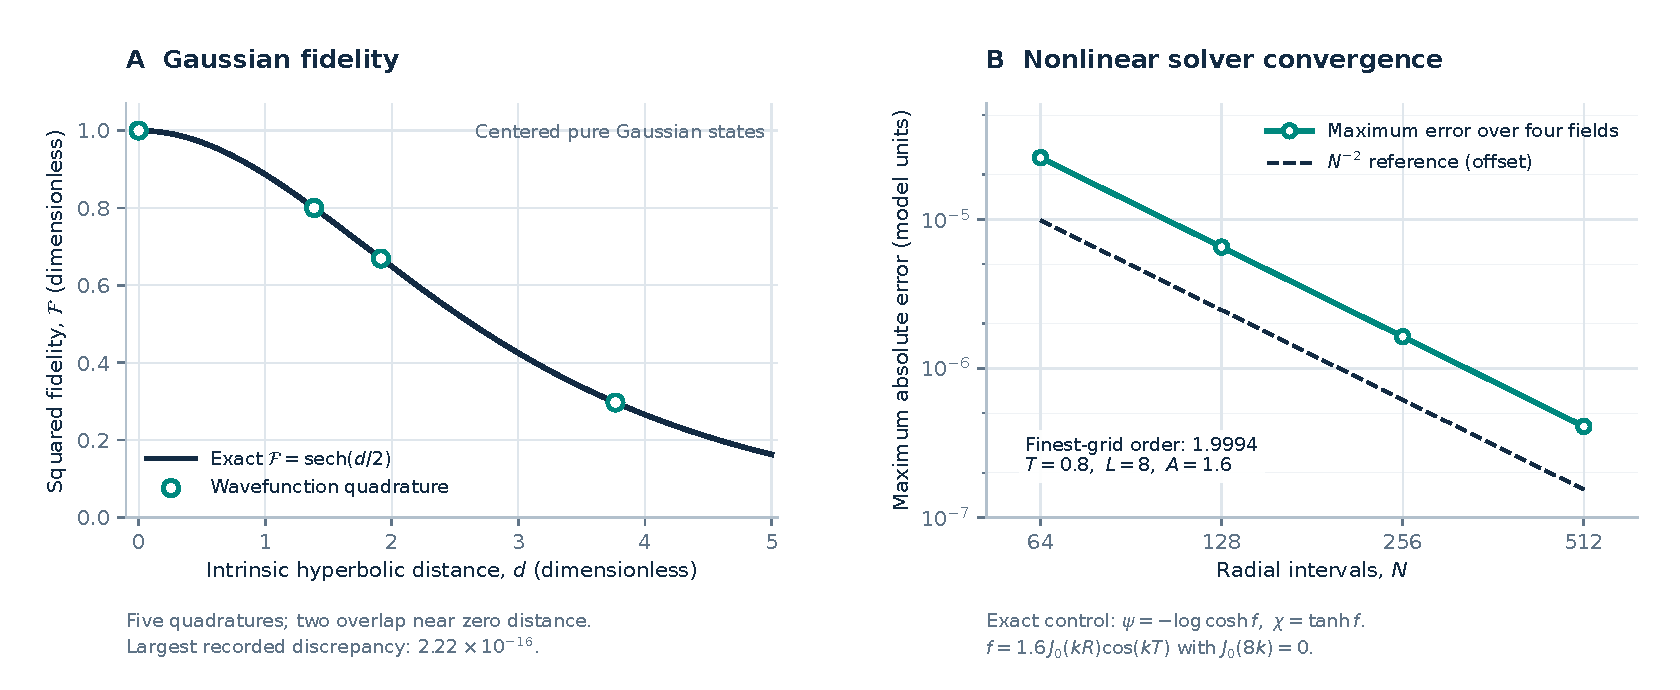
\includegraphics[width=\textwidth]{../figures/verification.pdf}
\caption{Independent finite checks. Left: the exact squared-fidelity curve and direct wavefunction quadratures; two near-zero-distance points overlap. Right: nonlinear geodesic/Bessel oracle errors against grid resolution, with a second-order reference guide. Both panels use synthetic mathematical data.}
\label{fig:checks}
\end{figure}

\section{Evidence, formal coverage, and reproduction}
The evidence types are intentionally distinct:
\begin{center}
\small
\begin{tabular}{@{}p{0.29\textwidth}p{0.65\textwidth}@{}}
\toprule
Evidence & Completed result and scope\\\midrule
Lean & 48 theorems in eight modules, zero warnings and errors. Original 40 plus eight residual identities/bounds.\\
Original symbolic suite & 373 exact checks, including 256 Riemann components; 256 additional rational noncommuting-current cases.\\
Independent exact checks & 58 identities and sharpness/negative-control checks; five direct wavefunction quadratures.\\
Nonlinear computations & Seven corrected benchmark evolutions, two exact-solution grid families, and separate temporal refinement.\\
Physical observations & None supplied; operational applicability remains a hypothesis to test.\\\bottomrule
\end{tabular}
\end{center}
The formal build uses Lean 4.19.0 and the pinned mathlib revision
\begin{quote}\small\ttfamily
c44e0c8ee63ca166450922a373c7409c5d26b00b.
\end{quote}
All 48 axiom reports are limited to \texttt{propext}, \texttt{Classical.choice}, and \texttt{Quot.sound}. Warnings are treated as errors, and the successful research build has neither. A true proposition compiles; an intentionally false $0=1$ proposition is rejected in a separately labeled negative-control log.

Lean certifies its actual statements and assumptions. The original analytic bridge links explicit chart-equation hypotheses to genuine derivative hypotheses and connected-domain constancy. The full differential-geometric variation, state-reconstruction argument, and physical interpretation have written proofs and symbolic checks; they are not all encoded as Lean theorems. The Gaussian extensions and integrated near-affine bounds are likewise written derivations with independent checks. The eight new formal lemmas certify the pointwise residual foundation.

The scientific reference environment is Python 3.12.13, SymPy 1.14.0, NumPy 2.3.5, and SciPy 1.17.0. After installing the pinned requirements, the command
\begin{quote}\small\ttfamily
python scripts/reproduce.py --output-dir work/reproduction
\end{quote}
runs the bounded scientific checks without changing the archived evidence. The formal verifier is
\begin{quote}\small\ttfamily
python scripts/verify\_lean.py --project formal --output work/lean
\end{quote}
after fetching the pinned toolchain, dependencies, and cache. The repository includes exact commands, raw states, CSVs, logs, source hashes, and GitHub Actions workflows. Hashes establish byte identity, not external replication or physical truth. The independent review pass was separately tasked AI work, not external peer review.

\section{Interpretation and next obligations}
The result is an exact meeting point between quantum phase-space geometry and a nonlinear gravitational model. The coefficient family is selected within the declared theory class, and the quantum metric, finite overlap, and geometric phase have explicit common formulas. Quantitative residual bounds make the calibration argument usable with imperfect computation.

The frame and derivative assumptions matter. Ricci-flat backgrounds remain stationary for broad curvature-squared additions; vacuum calibration alone therefore cannot rule out every higher-derivative completion~\cite{Pravda}. The source provides a curved Levi-Civita discriminator for one specified reduced deformation. A minimal massive or nonzero-orbit-momentum probe can identify the literal quotient frame under calibrated coupling and normalization. Such existence constructions do not constitute measurements.

The next mathematical obligations are a controlled interacting quantum continuum, its renormalization and physical constraints, and extension beyond the two-symmetry sector. Reduced-gravity renormalization work~\cite{Niedermaier} supplies relevant precedent, not proof of convergence for this package's regulated constructions. The next numerical obligations are longer and broader independently controlled evolutions. The next operational obligations are independently calibrated probes and measurements that test the physical dictionary.

The finite-distance and Berry formulas are exact specializations of established quantum geometry, newly made explicit in this model. The calibration route and verification package are presented with their precise assumptions; worldwide novelty is not established by this bounded literature comparison. The value of the release is a clear mathematical claim with a checkable route from assumptions to conclusions.

\section*{Availability and attribution}
Research by Logan Voss, with AI-assisted derivation, checking, formalization, and editing. The GitHub bundle preserves the original v2.4 supplement, the recovered v2.3 archive and earlier lineage, current source code, and newly executed evidence. Rights and dependency notices accompany the repository.

\begin{thebibliography}{10}
\bibitem{Voss24} L. Voss research program, \emph{Chart Selection, Variational Closure, and Integrability}, verification supplement v2.4, 12 November 2026. Preserved in \texttt{source/v2.4/} with manuscript, derivations, and execution receipts.
\bibitem{Banchi} L. Banchi, S. L. Braunstein, S. Pirandola, \emph{Quantum fidelity for arbitrary Gaussian states}, Phys. Rev. Lett. 115, 260501 (2015). \url{https://arxiv.org/abs/1507.01941v1}.
\bibitem{Garcia} A. Garcia-Chung, \emph{On the geometric phase for Gaussian states} (2020). \url{https://arxiv.org/abs/2004.14204v1}.
\bibitem{Seshadri} S. Seshadri, S. Lakshmibala, V. Balakrishnan, \emph{Geometric phases for generalized squeezed coherent states}, Phys. Rev. A 55, 869 (1997). \url{https://arxiv.org/abs/quant-ph/9905101v1}.
\bibitem{Cruz} J. Cruz, A. Mikovi\'c, J. Navarro-Salas, \emph{Free Field Realization of Cylindrically Symmetric Einstein Gravity}, Phys. Lett. B 437, 273--278 (1998). \url{https://arxiv.org/abs/gr-qc/9802067v3}.
\bibitem{Grumiller} D. Grumiller, W. Kummer, D. V. Vassilevich, \emph{Dilaton Gravity in Two Dimensions}, Phys. Rept. 369, 327--430 (2002). \url{https://arxiv.org/abs/hep-th/0204253v9}.
\bibitem{Hoare} B. Hoare, N. Levine, A. A. Tseytlin, \emph{Sigma models with local couplings: a new integrability--RG flow connection}, JHEP 11, 020 (2020). \url{https://arxiv.org/abs/2008.01112v3}.
\bibitem{Nicolai} H. Nicolai, D. Korotkin, H. Samtleben, \emph{Integrable Classical and Quantum Gravity} (1996). \url{https://arxiv.org/abs/hep-th/9612065v1}.
\bibitem{Pravda} V. Pravda, A. Pravdov\'a, J. Podolsk\'y, R. \v Svarc, \emph{Exact solutions to quadratic gravity}, Phys. Rev. D 95, 084025 (2017). \url{https://arxiv.org/abs/1606.02646v3}.
\bibitem{Niedermaier} M. Niedermaier, \emph{Dimensionally reduced gravity theories are asymptotically safe}, Nucl. Phys. B 673, 131--169 (2003). \url{https://arxiv.org/abs/hep-th/0304117v1}.
\end{thebibliography}
\end{document}
